\documentclass[11pt]{article}

% ---------- Packages ----------
\usepackage[margin=1in]{geometry}
\usepackage{amsmath, amssymb, amsthm}
\usepackage{graphicx}
\usepackage{float}
\usepackage{booktabs}
\usepackage{hyperref}
\usepackage{enumitem}
\usepackage{tikz}
\usetikzlibrary{positioning}

% ---------- Title Info ----------
\title{EECS 491 Assignment 3}
\author{JPF85}
\date{\today}

% ---------- Convenience Macros ----------
\newcommand{\E}{\mathbb{E}}
\newcommand{\Z}{\mathcal{Z}}
\newcommand{\neigh}{\mathrm{ne}}
\newcommand{\dd}{\mathrm{d}}

\begin{document}
\maketitle

\section{Exercise 1: MRFs and Image Denoising (40 pts)}

\subsection{1.1  Derive the equation that specifies the change in the energy equation when one variable changes state.}
\noindent \textbf{\underline{Concepts}}\\
Markov Random Fields\\
Energy minimization\\
\noindent \textbf{\underline{Tutorial}}\\
This question was pretty easy, just remeber that you are calculating a change in energy so you are subtracting the energy equation of "flipped" x from that of the 
 origonal x.  Then you just do some simple algebra, summations almost all cancel out unless they rely directly on x and x', and x' = -x so this is also useful for
 simplifying.\\
\noindent \textbf{\underline{Answer}} \\We need to derive the equation for $\delta\,E$, which can be derived by taking the difference between the Energy (E) calculated with your base value of x
 and the Energy with x being flipped.  Since x has two states we can say our fipped x is equal to -x, which allows us to easily simplify as so.
\begin{align*}
    \delta\,E   &= E(x',y) - E(x,y) && \text{where x' is flipped x, x' = -x}\\
                &= h(-2x) - \beta\sum_{j \in ne(x)}(-2x\,x_{j}) - \eta(-2x\,y) && \text{Terms Cancel if they do not depend on x', replace x' with -x}\\
                &= -2hx + 2\beta\,x\sum_{j \in ne(x)}(x_{j}) + 2x\,y && \text{simplify}\\
                &= 2x(\eta\,y + \sum_{j \in ne(x)}x_{j} - h)
\end{align*}

\subsection{1.2 Write a program to iteratively (or in random order) update the state variables to minimize the energy
(maximize the probability). Explain the design of your code.}
\noindent \textbf{\underline{Concepts}}\\
coding\\
\noindent \textbf{\underline{Tutorial}}\\
This was really easy, once you have the equation just slap it into some code, just make sure to handle the edges of the matrix correctly and load the matrix well (all 1 or -1).\\
\noindent \textbf{\underline{Answer}} My approach is to first convert the black and white image to a matrix of 1 (black pixel) or -1 (white pixel) then iterate over every pixel, see if swapping it
 to the other state will reduce the energy, if it does then flip the pixel and move on if it doesn't then don't change the pixel and move on.  My plan is to go through the
 image matrix row by row, not randomly, although it is possible that a randomized algorithm would reach the energetic minimum faster.  Code in Q1.py.  Turns out randomizing
 really helps so I actually swiched to doing this.\\

\subsection{1.3 Convergence plot: Energy vs passes (5 pts)}
\noindent \textbf{\underline{Concepts}}\\
coding\\
\noindent \textbf{\underline{Tutorial}}\\
just make sure you save the change in energy at each pass then plot it.\\
\begin{figure}[H]
    \centering
    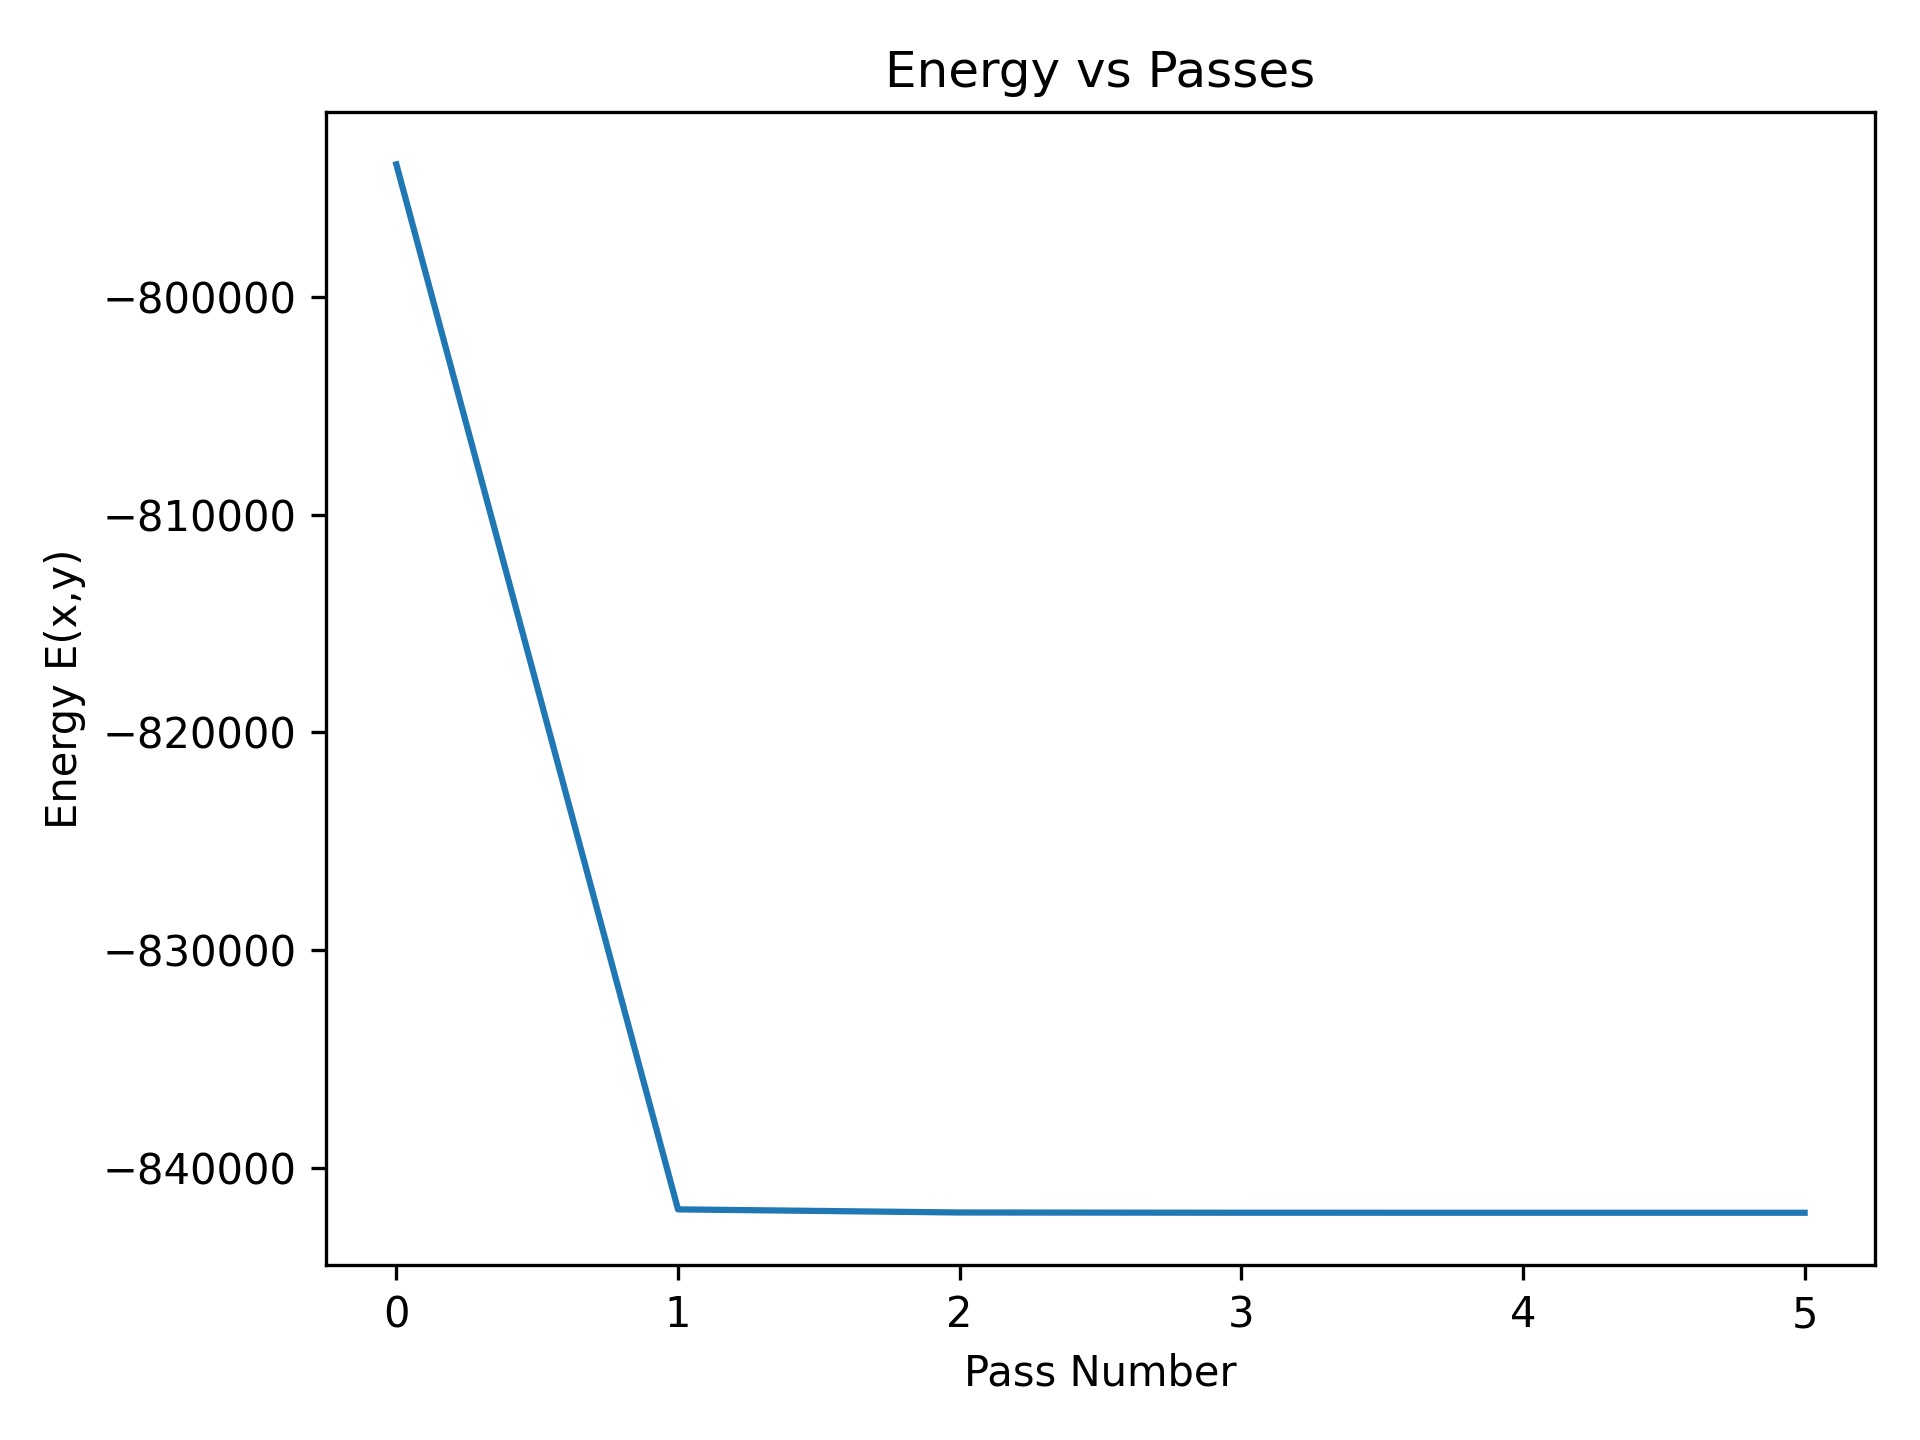
\includegraphics[width=0.6\textwidth]{Q1P3.png}
    \caption{Energy vs number of passes through pixels.}
\end{figure}

\subsection{1.4 Denoised image snapshots (5 pts)}
\noindent \textbf{\underline{Concepts}}\\
coding\\
\noindent \textbf{\underline{Tutorial}}\\
just make sure you save the image at start mid and end then plot it.\\
\\noindent \textbf{\underline{Answer}} The origonal figure is Grid.jpg\\
\begin{figure}[H]
    \centering
    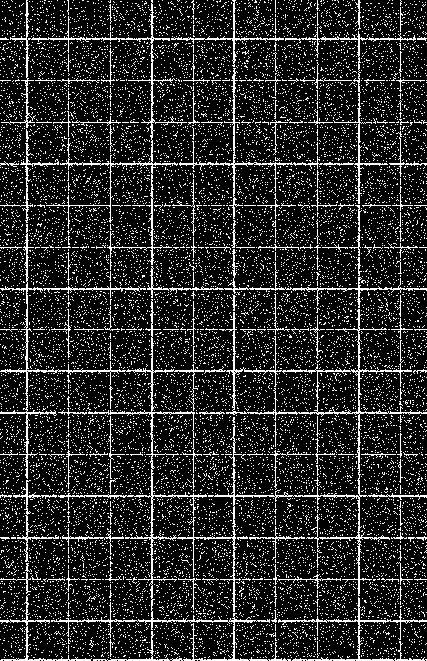
\includegraphics[width=0.6\textwidth]{denoise_start.png}
    \caption{Starting, noisy image}
\end{figure}
\begin{figure}[H]
    \centering
    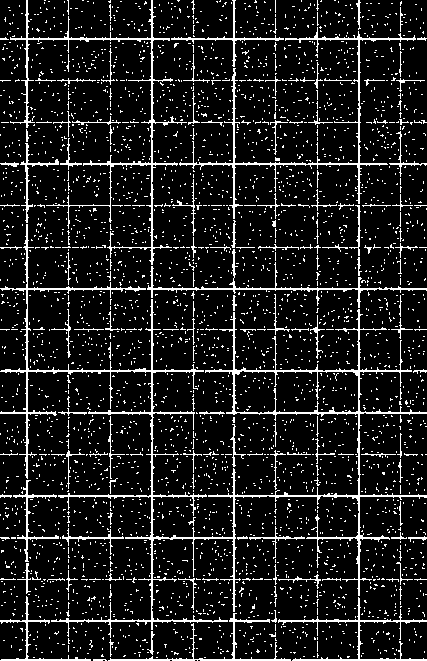
\includegraphics[width=0.6\textwidth]{denoise_half.png}
    \caption{halfway noise removed}
\end{figure}
\begin{figure}[H]
    \centering
    \includegraphics[width=0.6\textwidth]{denoise_end.png}
    \caption{final denoised image}
\end{figure}
\subsection{1.5 Parameter experiments (5 pts)}
\noindent \textbf{\underline{Concepts}}\\
n/a\\
\noindent \textbf{\underline{Tutorial}}\\
n/a\\
\noindent \textbf{\underline{Answer}} When looking at parameters for the energy equation we have our three: beta which controls how smooth the data is, how much noise is preserved vs how
 much smoothing to implement.  A higher beta encourages srtong smoothing, but can result in losing small details while a low beta has the opposite effect, retains
 more noise but also does not jepordize small features.  The second parameter is eta, which controls how much to "trust" the origonal noisy image.  A higher eta
 will mean that you want to trust the input a lot, which results in less denoising and more maintinance of small details that might be removed by the noise reduction
 with a larger eta.  The final parameter we can tune is h, which corrosponds to a global bias to black (1) or white (-1).  A negative value of h biases toward a more
 white image and a positive value biases toward a more black image, this is less a choice between removing noise vs retaining small features as the other parameters are
 and more a choice between wether you think the real image is primarily white or primarily black.\\

\subsection{1.6 Generalize the energy model (10 pts)}
\noindent \textbf{\underline{Concepts}}\\
Algorithm development\\
\noindent \textbf{\underline{Tutorial}}\\
Honestly I don't know, just think about what sort of images this doesn't work on.  My initail reaction is greyscale images or images that are not classifed as binary,
 so you would be looking at a difference in pixel values instead of just a 1/-1 agree/disagree relationship.  Just think of how each term would change if this was the
 case and work from there.\\
\noindent \textbf{\underline{Answer}} Instead of a binary black/white 1/-1 version of the problem what if the images were classified in color?  Or let's say greyscale
 for simplicity.  This takes our discrete system and makes it continous, so isntead of looking at agreement of neightboring pixels we are looking at difference in
 the color value.  This results in an adjusted equation:
\begin{align*}
    E(x,y)  &= \beta \sum_{(i,j) \in nb}(x_{i} - x_{j})^{2} + \eta \sum_{i} (x_{i} - y_{i})^{2} + h \sum_{i}x_{i}
\end{align*}
This is basically the exact same equation, we just use distance or difference measurements instead of seeing if pixels agree by multiplying them.  In the old model we
 would get a poistive value from mulitplying pixels if they agree, and a negative value if they disagree and subtract these values in order to find the minumum energy.  In
 the case of this new equation we still minimize energy, but the terms are added together this time so that we can look for the smallest differences instead of the maximal
 agreement.  This model also resembeles a gaussian markov random field for energy minimzation.\\
\section{Exercise 2: Graphical Representation (15 pts)}

\subsection{2.1 Convert given Bayes net to an MRF + potentials (5 pts)}

\noindent \textbf{\underline{Concepts}}\\
MRFs and potential functions\\
Bayes Nets\\
\noindent \textbf{\underline{Tutorial}}\\
For this question it is really just a matter of reviewing how to convert a Bayes net to a MRF.  All you have to do is connect any parents who share a child with a new edge,
 and then remove the directionality of each edge.  Then you just write the potential functions for all the maximal cliqes and multiply them together to get the joint
 probability.

\noindent \textbf{\underline{Answer}}\\
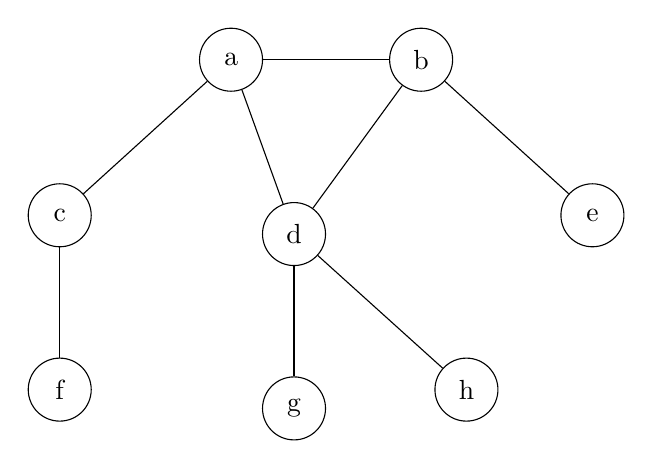
\begin{tikzpicture}[
  every node/.style={circle, draw, minimum size=8mm},
  node distance=14mm and 16mm
]
\node (a) {a};
\node (b) [right=of a] {b};

\node (c) [below left=of a] {c};
\node (d) [below=of a, xshift=8mm] {d};
\node (e) [below right=of b] {e};

\node (f) [below=of c] {f};
\node (g) [below=of d] {g};
\node (h) [below=of e, xshift=-16mm] {h};

\draw (a) -- (b);
\draw (a) -- (c);
\draw (a) -- (d);
\draw (b) -- (d);
\draw (b) -- (e);
\draw (c) -- (f);
\draw (d) -- (g);
\draw (d) -- (h);
\end{tikzpicture}
And the potentail function: \\
\begin{align*}
    p(a,b,c,d,e,f,g,h)  &= \prod_{Cliques}\\
                        &= \frac{1}{z}\phi(a,b,d)\phi(a,c)\phi(c,f)\phi(b,e)\phi(d,g)\phi(d,h)
\end{align*}
\subsection{2.2 Factor graph for the Bayes net (5 pts)}
\noindent \textbf{\underline{Concepts}}\\
Factor Graphs\\
Bayes Nets\\
\noindent \textbf{\underline{Tutorial}}\\
For this question it is really just a matter of reviewing factor graphs.  Basically they are just bipartite graphs where you generat a node in the bipartite graph for each
 node in the bayes net, and another node for each joint probability.  Then these joint probability nodes are used to connect parents to children and you just have to write
 out the joint probabilty using these factor functions, which are just $p(x \mid parents(x))$

\noindent \textbf{\underline{Answer}}\\

\subsection{2.3 Two different factor graphs for sprinkler Bayes net (5 pts)}


\section{Exercise 3: The Sum-Product Algorithm (20 pts)}

\subsection{3.1 Messages for the factor graph (5 pts)}
% Write all factor-to-variable and variable-to-factor messages symbolically.

\subsection{3.2 Marginal expression (5 pts)}
% Express the requested marginal in terms of messages.

\subsection{3.3 Verify marginal by substitution (5 pts)}
% Substitute message definitions and show it matches.

\subsection{3.4 Add a loop: consequences for sum-product (5 pts)}
% Discuss loopy belief propagation: convergence, exactness, when it can still be used.

\end{document}